\chapter{Climate Models}
\lastupdated{2024-12-13}{\chapterFourClimModOverleaf}
We will use the shallow water equation, but to have a realistic case, we need to put it on the sphere. We start from the usual equation, for convenience we introduce the geopotential $\Phi=gH$:
\begin{align}
	\frac{\partial u}{\partial t}=-u\frac{\partial u}{\partial x}-v\frac{\partial u}{\partial y}+fv-\frac{\partial \Phi}{\partial x} \\
	\frac{\partial v}{\partial t}=-u\frac{\partial v}{\partial x}-v\frac{\partial v}{\partial y}-fu-\frac{\partial \Phi}{\partial y} \\
	\frac{\partial \Phi}{\partial t}=-\frac{\partial u\Phi}{\partial x}-\frac{\partial v\Phi}{\partial y}
\end{align}
Let's use $U=u\cos\phi$, $V=v\cos\phi$, $\vec{V}=\hat{i}U+\hat{j}V$. Until now all the methods we have introduced are designed to give us instruments to simulate and march the atmosphere and the oceans and, probably, much more.
What is the difference between all these applications?
\begin{itemize}
	\item Forecast (the target is the instantaneous state of the system)
	      We start at a specific moment that we try to specify as accurately as we can and we want desperately to stay close to the state of the system for as long as we can.
	      Here the main forcing is the internal dynamic of the atmosphere and the ocean. The conservation properties becomes progressively more important as the range of the forecasts becomes longer.
	\item Climate (the target is the statistics of the system)
	      We want to reproduce its statistical distributions and the initial condition may not be so important, in fact we could start at rest.
\end{itemize}
Here the main forcing are the external forcing and the structure (composition) of the atmosphere and the ocean. Conservation properties are important. The question here is: what will be the state of the atmosphere and the ocean in where the initial conditions won't be independent?
\\


Both systems are affected by forcing, but in the forecast case there is no equilibrium.

\section{Radiative Model}
The Sun is the primary forcing and climate is the state in equilibrium with it.
Firstly then, we have to take into consideration the fact that there must be preserved balance between absorbed solar radiation and emitted planetary radiation.
To compute the absorbed radiation we have to take into consideration the Solar constant $S_{0}$ which is the energy per unit of area and time that reaches a perpendicular surface placed at a distance of 1 astronomical unit. Therefore, the energy incident on the planet is given by the product of the solar constant and the area that the planet exposes to the incident radiation perpendicularly to it (as shown in Figure \ref{fig: fig1}).
\begin{wrapfigure}{r}{0.18\textwidth}
	\begin{center}
		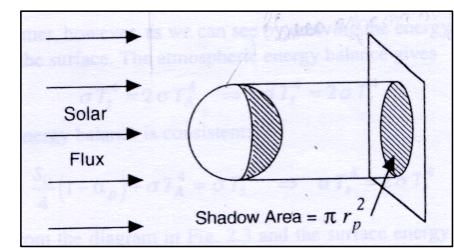
\includegraphics[width=0.30\textwidth]{uploads/47image.png}
	\end{center}
	\caption{Relationship between intensity}
	\label{fig: fig1}
\end{wrapfigure}
It is called shadow area and it is approximately $\pi R^2$ where R is the radius of the planet taken into consideration.
Given that the absorbed radiation is equal to $S_{0}= \pi R^2$
This absorbed radiation during all day is distributed along the entire planet, so along the entire sphere $4\pi R^2$; so that it becomes $$S_{0}= \frac{\pi R^2}{4\pi R^2}=\frac{S_{0}}{4}$$
Furthermore, it must be kept in mind that not all the incident radiation is absorbed; part of it will be reflected. The measure of a planet's reflectivity is called albedo.
So that $\frac{S_{0}}{4} (1-\alpha)$ is the real absorbed radiation.
The planetary albedo $a$ is about $0.3$, and the solar constant conventional value is $1361$ W/m$^2$


\begin{figure}[htpb]
	\centering
	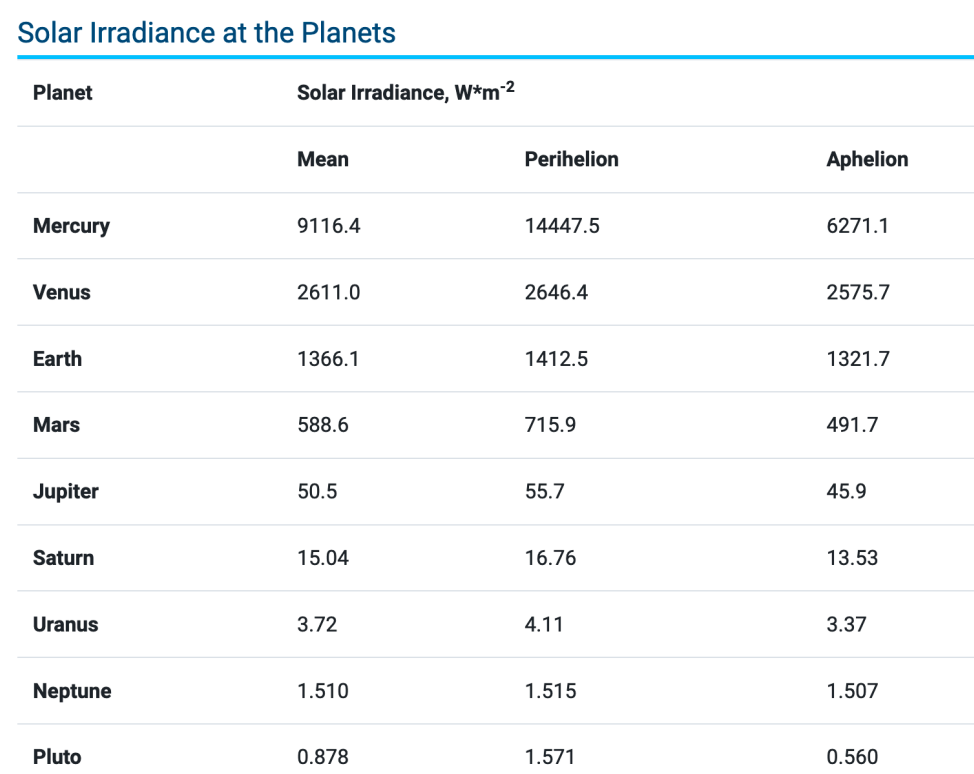
\includegraphics[width=0.35\linewidth]{uploads/Screenshot 2024-11-19 154224.png}
	\caption{Solar Irradiance at the Planets}

\end{figure}
then
\begin{align*}\label{eq1}
	F_S=\frac{S(1-a)}{4}                              \\
	\sigma T^4= \frac{S(1-a)}{4} \qquad\text{S-B Law} \\
	T=\left(\frac{S(1-a)}{4\sigma}\right)^{1/4}
\end{align*}
with $S=1361$, $a=0.3$ and $\sigma=5.67 \, \, 10^{-8}$, turns out that $T_S=254\text{K}=-18\text{°C}$.
From Stefan Bolzmann Law, $\sigma T^4$ is the emitted radiation by a blackbody at temperature $T$; as $T_S$ found this way is inaccurate, it can be concluded that the Earth-atmosphere system cannot be simply considered as a black body emitting at the temperature of the Earth's surface, since part of the emitted radiation is absorbed by the atmosphere itself. In this sense, the Earth's surface temperature does not reflect that of a black body in equilibrium with the incident solar radiation. However, the emission temperature obtained in this way is in good agreement with the temperature of the tropopause. The reason for this is that the tropopause represents the limit above which there is no significant absorption of infrared radiation, so the system, as seen from the tropopause, can indeed be approximated as a black body in terms of emission, in equilibrium with the incident solar radiation.

Satellite observations are giving us the observed long wave outgoing radiative flux
from the planet outside the atmosphere. In fact it is so detailed that we have seen this flux geographically distributed over the all surface. Its global average is $226\, \, \text{W/m}^2$ from ERA5. With the satellite observations, we can came up with an equation with the observed long wave outgoing radiative flux geographically distributed all over the surface. $OLR_{mean}$ stands for Outgoing Longwave Radiation, the thermal radiation emitted by Earth back into space. $OLR$ is a key component of the planetary energy balance, as it represents the primary way Earth loses heat to space. The amount of $OLR$ depends on the Earth's surface temperature, atmospheric temperature profile, and the presence of greenhouse gases.
We can use that flux to find the corresponding temperature:
$$\sigma T^4=OLR_{mean}\Longrightarrow T=\left(\frac{OLR}{\sigma}\right)^{1/4}$$
with $OLR=226$ and $\sigma=5.67 \,\, 10^{-8}$
hence, $T_S=251 \text{K}=-21\text{°C}$. This is still not the temperature at the surface, whose global, long term
mean is about $288$ K or $15$° C, it is though what the satellite sees: it's the level at which emission reaches the out space. There is something that is making the surface opaque, hence the satellite doesn't see the surface but a layer on a higher level (remember that $T$ decreases as the height increases).
Maybe the earth surface is not really a black body and not all the
radiation reaches outer space. Let us introduce a factor $\tau$, the transmissivity:
$$\tau\sigma T^4=OLR_{mean}$$
and calibrate $\tau$ with the observed surface temperature.
\begin{equation}\label{eq.tau}
	\tau=\left(\frac{OLR}{\sigma T_S^4}\right)\approx 0.58
\end{equation}
so the observed surface temperature can be explained only assuming that not all the radiation emitted from the surface reaches outer space. The level where the radiation is able to escape is above and it is cooler.

\begin{figure}[htpb]
	\centering
	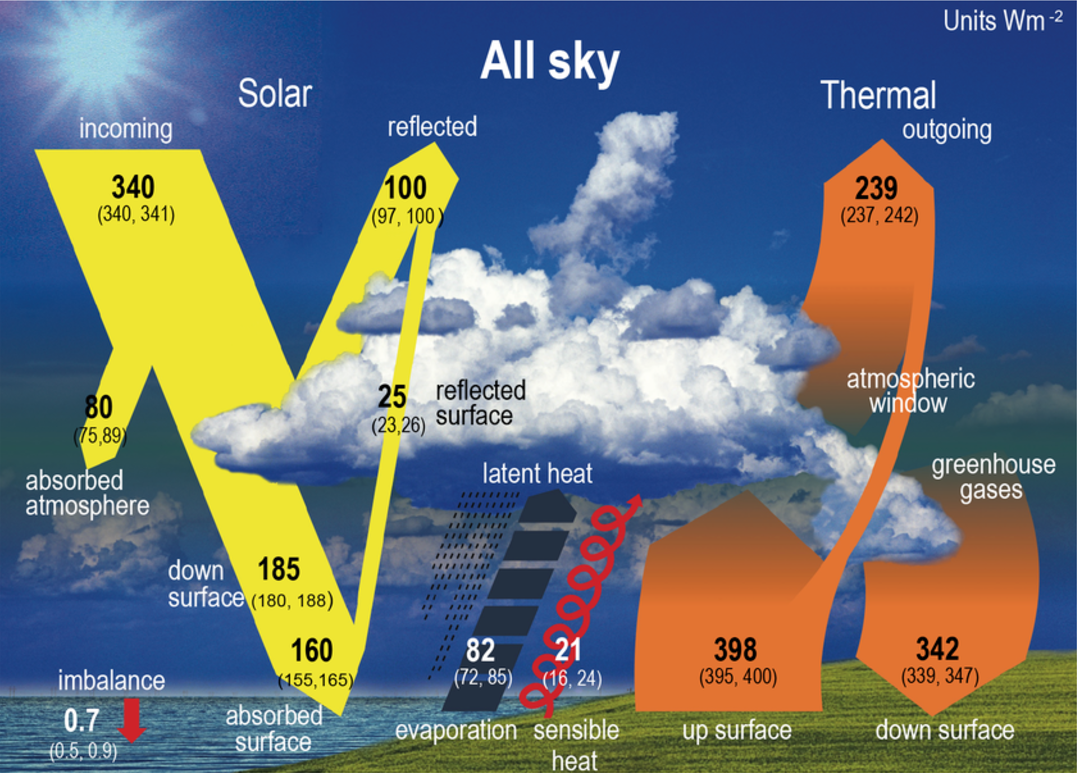
\includegraphics[width=0.5\linewidth]{uploads/Screenshot 2024-12-01 132204.png}
	\caption{Earth-atmosphere system energy balance}

\end{figure}
The two- and three-layer atmosphere models are simplified frameworks to study Earth's radiation balance and the greenhouse effect. They explain how energy flows between the surface, the atmosphere, and space.

In the two-layer model, the Earth's surface absorbs solar radiation and emits infrared radiation, which is partially absorbed and re-emitted by greenhouse gases in the atmosphere. This re-emission back toward the surface enhances warming, maintaining an energy balance where incoming solar energy equals outgoing infrared radiation.

The three-layer model adds complexity by including an upper atmospheric layer (e.g., stratosphere), where radiation escapes to space. It considers energy transfer between the surface, middle atmosphere (troposphere), and upper atmosphere, capturing how each layer absorbs, emits, and redistributes radiation. The effective radiating level (ERL)—the altitude from which most radiation escapes to space—shifts higher with increased greenhouse gases, warming the surface while cooling upper layers.


These models illustrate key processes like vertical temperature profiles, with temperatures decreasing with altitude in the troposphere; radiative-convective equilibrium, balancing energy absorption, emission, and convection. They also depict climate sensitivity, showing how increased greenhouse gases amplify the greenhouse effect and raise surface temperatures.
By simplifying Earth's energy flows, these models provide insights into how atmospheric layers interact and how greenhouse gases affect global warming.
\subsection{Two-layer atmosphere}
We need both the in flux and the out flux to be at balance: assuming that the atmosphere is transparent so no change in $S$ is caused by the atmosphere, we have the following equations for atmospheric balance:
\begin{equation}\label{eq.two layer}
	(1-\alpha)S=4\sigma T^4_{a}+4(1-\tau)\sigma T_S^4
\end{equation}
$\alpha$ is the albedo, $\tau$ is transmissivity. The equation for the surface balance is:
\begin{equation}\label{eq.surface balance}
	\epsilon (1-\alpha)S+4\sigma T_a^4=4\sigma T_S^4
\end{equation}
where $\epsilon$ is a factor accounting for possible absorption of the atmosphere at solar radiation, $(1-\alpha)S$  is carried from the atmosphere, $4\sigma T_a^4$ is emitted by the atmosphere and $4\sigma T_S^4$ emitted by the surface.
$T_a$ is the atmospheric temperature and $T_S$ the surface temperature.


In the equation for the surface balance we account for two fluxes: one coming from the Sun, attenuated by a factor $\epsilon$, another coming from the atmosphere radiating downward (see the fig\ref{fig:two layer}).
Hence,
\begin{equation}
	\left(F_S=\frac{S\alpha\epsilon+S\alpha-S\epsilon-S}{4\tau-8}, F_a=\frac{S\alpha\epsilon\tau-S\alpha\epsilon+S\alpha-S\epsilon\tau+S\epsilon-S}{4\tau-8}\right)
\end{equation}
this the solution in terms of the fluxes.
\begin{figure}[h!]
	\centering
	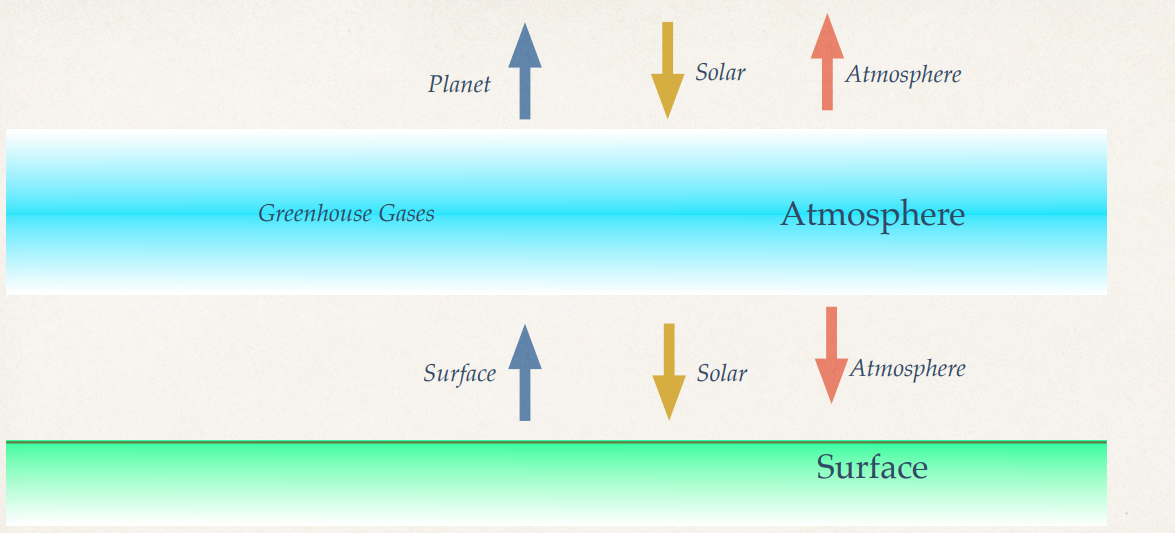
\includegraphics[width=0.5\linewidth]{uploads/Screenshot 2024-11-20 114831.png}
	\caption{Two-layer atmosphere}
	\label{fig:two layer}
\end{figure}
Lets’ look at different situations.
\begin{enumerate}
	\item First assume the atmosphere does not absorb the solar radiation ($\epsilon =1$): the atmosphere is totally transparent to solar radiation; and the transmissivity of the atmosphere is 0.0, no emission from the atmosphere:
	      $$F_S=\frac{S(1-\alpha)}{4}=238 \,\text{W/m}^2 \,\,\text{and}\,\, F_a=0$$
	      that is the same balance as before when we didn't account for atmosphere
	\item Let’s allow now for some absorption of terrestrial radiation and the transmissivity of the atmosphere is 0.5:
	      $$F_S= 396 \,\text{W/m}^2 \quad F_a=158 \, \text{W/m}^2$$
	      $$T_S= 289 \,\text{K}\approx 15\text{°C} \quad T_a=230 \, \text{K}\approx -43\text{°C}$$
	      meaning that even with less than 0.5, the presence of atmosphere will give $T$ above 0°C. Opacity of the atmosphere is what makes possible the liquid water.
	\item Assume a very opaque atmosphere the transmissivity is 1.0:
	      $$F_S=476 \,\text{W/m}^2 \quad F_a=238 \, \text{W/m}^2$$
	      $$T_S= 302 \,\text{K}\approx 28\text{°C} \quad T_a=254 \, \text{K}\approx -19\text{°C}$$
\end{enumerate}


\textcolor{RoyalBlue}{Opacity}: it refers to the degree to which the Earth's atmosphere prevents certain wavelengths of radiation (typically infrared radiation) from passing through it. This concept is closely connected to the greenhouse effect, as atmospheric opacity governs how much outgoing longwave radiation from the Earth's surface is absorbed and re-emitted by greenhouse gases. Greenhouse gases, such as carbon dioxide ($CO_2$), water vapor ($H_2O$), methane ($CH_4$), and others, absorb infrared radiation emitted by the Earth's surface.
The atmospheric opacity at certain infrared wavelengths increases with the concentration of these gases, preventing radiation from escaping to space.
This absorption and re-emission process warms the Earth's surface and lower atmosphere. \\


Climate models use radiative transfer equations to simulate how variations in atmospheric opacity affect surface temperature, vertical temperature profiles, and energy transport.
\subsection{Three-layer atmosphere}
%If you are in continuous conditions the net flux between the fluxes up and down and the heating is proportional to the flux divergent that is the net balance between the 2 level is different
\begin{figure}[htpb]
	\centering
	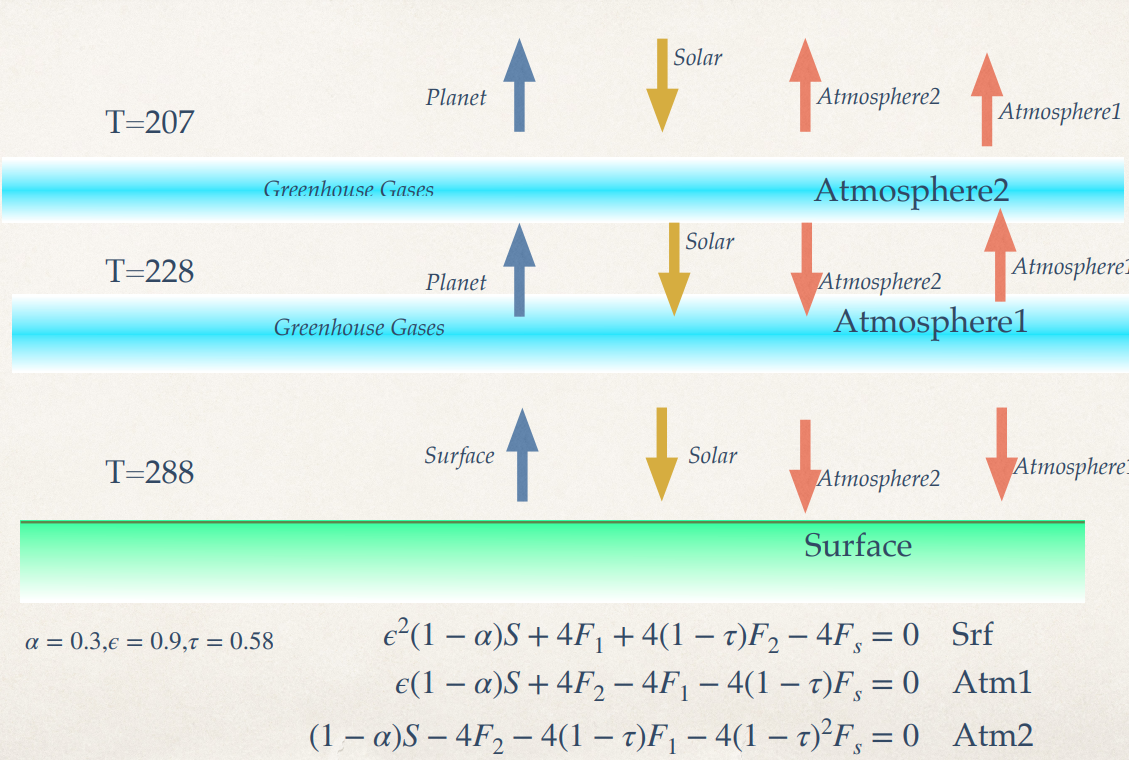
\includegraphics[width=0.55\linewidth]{uploads/Screenshot 2024-11-20 121339.png}
	\caption{Three-level atmosphere flux balance}
	\label{fig:three level}
\end{figure}
Remembering Kirchhoff’s law (the emissivity and absorptivity of a real surface are equal for radiation with identical temperatures and wavelengths), we
can introduce the temperature relations, we still consider the surface as a
black body: $$F_S=\sigma T^4 \,\,\, F_1=\tau\sigma T_1^4 \,\,\, F_2=\tau\sigma T_2^4$$
\paragraph{Radiative equilibrium} The transfer equation describes the behavior in the continuous case:
$$\frac{dF^{\downarrow}}{d\tau}=B-F^{\downarrow} \qquad  \frac{dF^{\uparrow}}{d\tau}=F^{\uparrow}-B$$
where $B=\sigma T^4$ is the blackbody emission, $\tau$ the optical depth linked to the geometric height by $d\tau=-e_Ldz$. If we are in continuous conditions the net flux is $N=F^{\uparrow}-F^{\downarrow}$ and the long wave heating is proportional to the net flux divergence $-\frac{\partial N}{\partial z}$. So,
$$\frac{d}{d\tau}F^{\downarrow}e^{\tau}=Be^{\tau}\quad \frac{d}{d\tau}F^{\uparrow}e^{-\tau}=-Be^{-\tau}$$
At equilibrium there is no radiative heating, so:
$$\frac{\partial}{\partial z}(F^{\uparrow}-F^{\downarrow})=0\rightarrow\frac{\partial}{\partial\tau}(F^{\uparrow}-F^{\downarrow})$$
in general this is not satisfied because the air is in motion, but suppose that such equilibrium exist, then the incoming solar radiation is balanced by OLR, $F^{\uparrow}_T=F^{\uparrow}(\tau=0)=S$, so we get the boundary conditions at the top:
$$F^{\downarrow}=0 \quad F^{\uparrow}=F^{\uparrow}_T \quad \text{at} \, \, \tau=0$$
\begin{figure}[htpb]
	\centering
	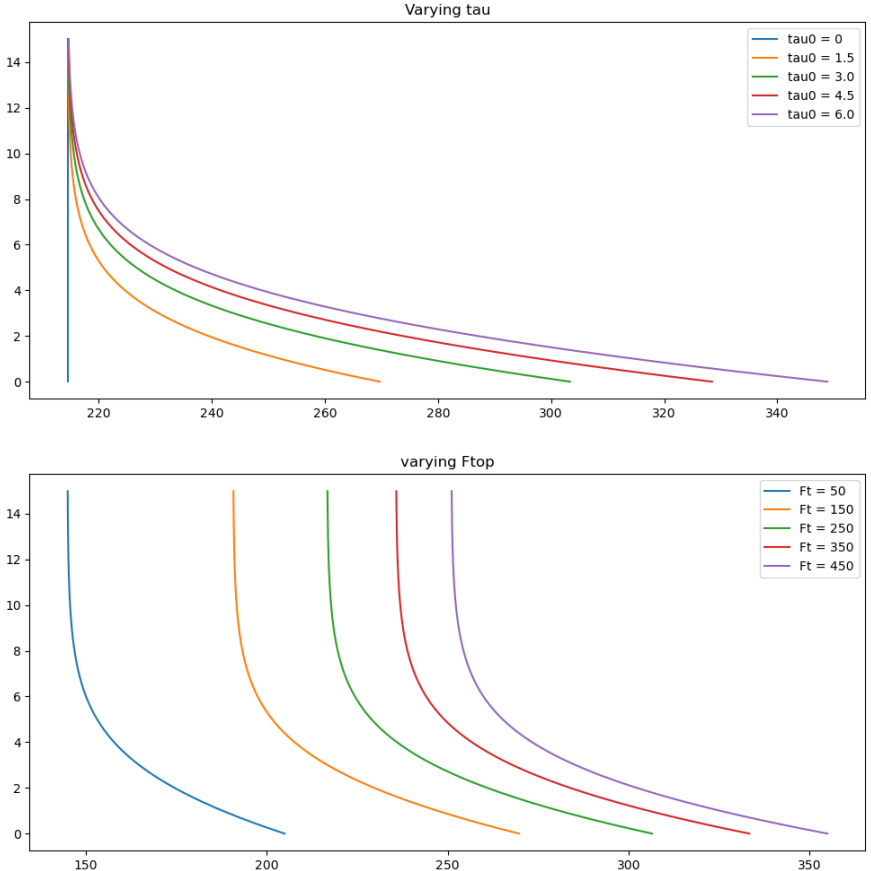
\includegraphics[width=0.5\linewidth]{uploads/Screenshot 2024-11-20 125556.png}
	\caption{The change in $OLR$}
	\label{fig:change in OLR}
\end{figure}




then the solution is
$$F^{\downarrow}=\frac{\tau}{2}F^{\uparrow}_T \quad F^{\uparrow}=(1+1/\tau )F^{\uparrow}_T \quad B=\frac{(1+\tau)}{2}F^{\uparrow}_T $$
The contribute from each level OLR is:
$$OLR_S=(1-\tau)^2\sigma T^4_S \qquad OLR_1=\tau(1-\tau)\sigma T_1^4 \qquad OLR_2=\tau\sigma T_2^4$$
add perturbation (change a little bit the opacity)
$$OLR_S=(1-\tau-\Delta\tau)^2\sigma T^4_S \qquad OLR_1=(\tau+\Delta\tau)(1-\tau-\Delta\tau)\sigma T_1^4 \qquad OLR_2=(\tau+\Delta\tau)\sigma T_2^4$$
we'll get different curves with different temperature.

Computing the change in $OLR$:
$$\Delta OLR_S\approx\Delta\tau[-2(1-\tau)]\sigma T_S^4 \qquad \Delta OLR_1\approx\Delta\tau(1-2\tau)\sigma T_1^4 \qquad \Delta OLR_2=\Delta\tau\sigma T_2^4$$
When greenhouse gas concentrations increase, the atmosphere becomes more opaque to infrared radiation, this reduces $OLR$ escaping to space at the top of the atmosphere. The difference between the before and after state of $OLR$ due to increased opacity is the \textit{radiative forcing}:
\begin{equation}\label{eq.radiative forcing}
	R\approx-\Delta OLR
\end{equation}
Radiative forcing describes how changes in atmospheric composition (opacity) affect the Earth's radiation budget by altering $OLR$. It quantifies the change in Earth's energy balance caused by a specific perturbation, such as an increase in greenhouse gases. The reduction of $OLR$ due to higher greenhouse gas opacity leads to positive radiative forcing, indicating an energy surplus, initiating global warming and affecting the climate system through feedback mechanisms; while negative radiative forcing results in cooling. \\


Radiative forcing initiates changes in Earth's climate system, which are then amplified or dampened by feedback mechanisms, such as the water vapor feedback (positive). The relationship between radiative forcing and global temperature change is encapsulated in the concept of climate sensitivity, often expressed as the temperature increase for a doubling of $CO_2$ (see later on).

\begin{figure}[htpb]
	\centering
	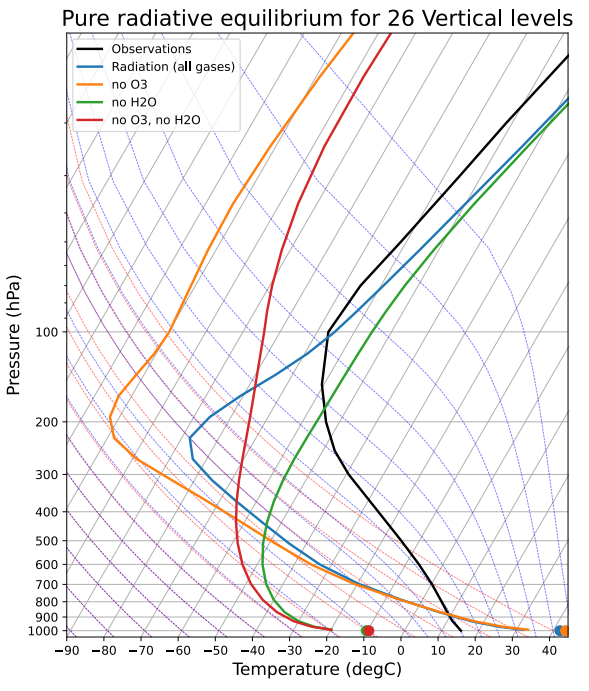
\includegraphics[width=0.30\linewidth]{uploads/Screenshot 2024-11-20 130113.png}

	\caption{the black line corresponds to the observations; the blue to the component of the atmosphere, it decreases with $T$ but in the stratosphere it changes inclination; the orange is without the ozone, responsable for the change of the slope in the stratosphere; the green one is without the water meaning that most of the opacity of the atmosphere disappears suddently, at the bottom $T$ is very cold; red without ozone and water, isotherm basically there is no atmosphere.}
	\label{fig:fig2}
\end{figure}


What about if we consider atmosphere composed by many more layers?
In Figure \ref{fig:fig2} is shown a radiative equilibrium for 26 levels, with a realistic radiation calculation and observed components gases, with transmissivity and absorption coefficients ($T$ profile with vertical coordinate $p$).

\section{Radiative-Convective Model}
\subsection{Radiative convective equilibrium}\label{subsec:convection adjustments}
\paragraph{Convection}
\begin{figure}[htpb]
	\centering
	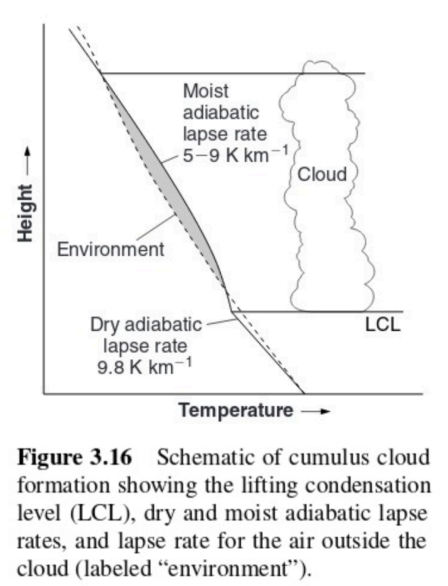
\includegraphics[width=0.28\linewidth]{uploads/Screenshot 2024-11-20 130640.png}\quad 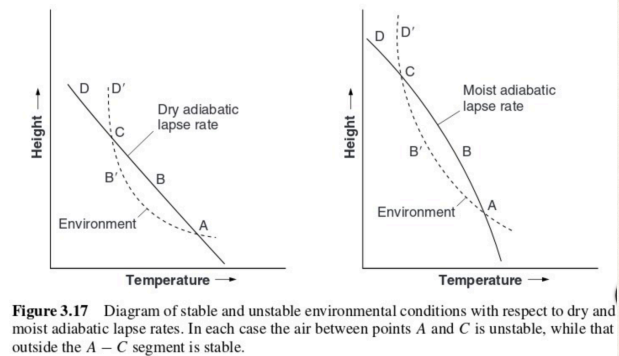
\includegraphics[width=0.5\linewidth]{uploads/Screenshot 2024-11-20 130727.png}
	\caption{Schematic representation of convection}

\end{figure}
Convection is about low layer mixing until they are gravitationally stable.

How to treat convection? Basically three steps:
\begin{enumerate}
	\item Identify the unstable layers;
	\item Look at the temperature and moisture profiles;
	\item Adjust until the profile is stable $\rightarrow$ conserve the energy distributing it vertically.
\end{enumerate}
Radiative-convective equilibrium is a simplified framework for understanding the balance between radiative processes and convection in the atmosphere. The goal of this framework is to describe how the atmosphere redistributes energy vertically to achieve balance between the incoming solar radiation and $OLR$. In the troposphere for example convection plays a dominant role in redistributing heat, while radiation becomes the primary mechanism in the stratosphere.


To incorporate convection into a radiative model, we consider temperature and moisture profiles. Let  $T_r$, $q_r$ be the equilibrium (reference) profiles for temperature and moisture. If the actual profiles $T_i$ and $q_i$ deviate from these references, the energy imbalance in the system can be calculated as:
\begin{align*}
	\int_{p_B}^{p_T}c_p(T_r-T_i)dp \qquad \text{temperature imbalance} \\
	\int_{p_B}^{p_T}c_p(q_r-q_i)dp \qquad \text{moisture imbalance}
\end{align*}

where the integration is over the pressures from the bottom to the top of the convective layer.
These expressions quantify the excess energy in the column relative to equilibrium, based on deviations in temperature and moisture. \\

If precipitation occurs, the total enthalpy (the sum of sensible and latent heat) in the system is conserved, and it is expressed as:
$$\int_{p_B}^{p_T}c_p(h_r-h_i)dp \qquad h=c_pT+Lq$$
where $L$ is the latent heat of vaporization. This conservation principle ensures that the redistribution of heat and moisture by convection does not alter the total energy content of the system. The vertical profiles are adjusted iteratively to stabilize the atmosphere. Before saturation, the temperature follows the dry adiabatic lapse rate, which describes how air cools as it expands. After saturation, the temperature follows the moist adiabatic lapse rate, which is slower because latent heat is released during condensation. Convective adjustment uses these principles to progressively bring the system closer to stability, ensuring that unstable layers are stabilized while conserving total enthalpy.


In the Radiative-Convective Equilibrium framework, convection and radiation interact to bring the atmosphere into equilibrium. This model provides a framework to understand how the atmosphere maintains energy balance. Convection redistributes energy vertically to stabilize the atmosphere, while radiation handles the energy exchange with space. The interplay between these processes is critical for maintaining the observed thermal structure of the atmosphere, particularly in the troposphere.


\begin{figure}[htpb]
	\centering
	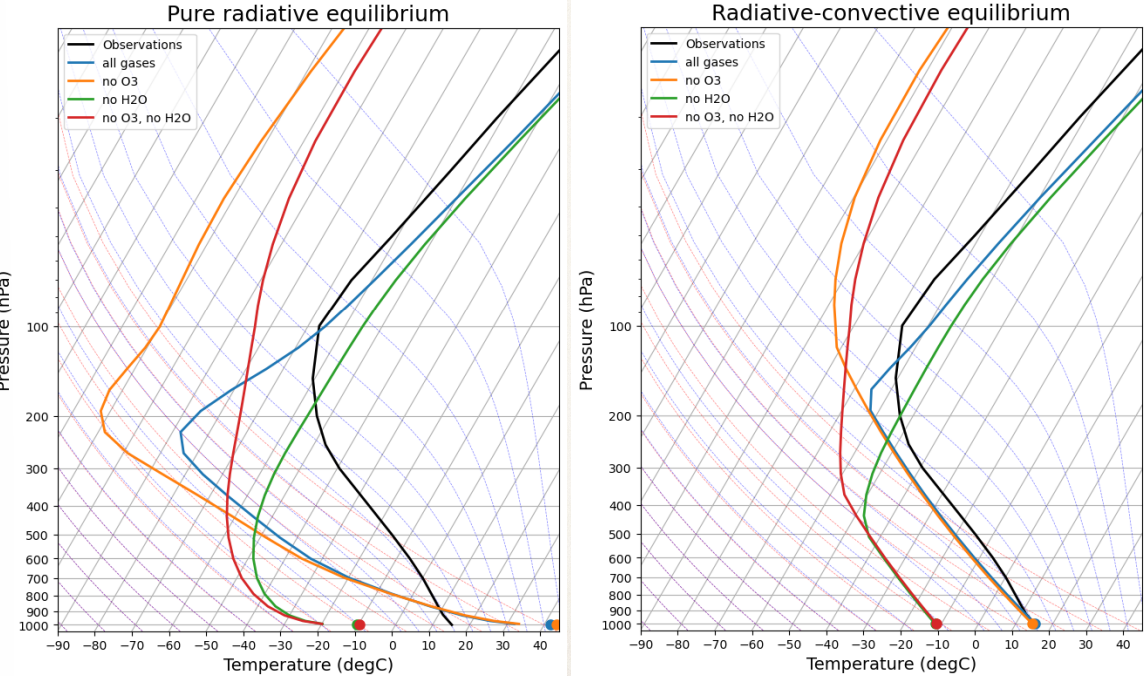
\includegraphics[width=0.5\linewidth]{uploads/Screenshot 2024-11-20 131319.png}
	\caption{Radiative Convective equilibrium}

\end{figure}
\section{Radiative forcing}
Radiative forcing measures the change in energy balance in the Earth's climate system due to external factors (forcings). It quantifies the difference between the incoming solar radiation absorbed by the Earth and the outgoing infrared radiation emitted back to space.


Radiative forcing is a commonly used metric for assessing climate change mechanisms: compared to calculations of surface temperature change, it is a relatively straightforward calculation. It allows a more quantifiable and robust comparison of climate change mechanisms between models. The adjusted radiative forcing has been adopted by the Kyoto Protocol and IPCC (Intergovernmental Panel on Climate Change) process; they defined it as \textit{‘the change in net irradiance at the tropopause after allowing stratospheric temperatures to readjust to radiative equilibrium’}. The global-mean radiative forcing ($\Delta R$) can be simply related to the equilibrium global-mean surface temperature change ($\Delta T$) by the simple formula $\Delta T=\lambda\Delta R$ which $\lambda$ is the climate sensitivity parameter.\\


RF is defined also as the instantaneous perturbation in net radiative flux at the tropopause exerted by a change in a component of the radiative budget,
with surface temperature and tropospheric state maintained in their
unperturbed state. The term “radiative forcing” has been employed in the IPCC Assessments to denote an externally imposed perturbation in the radiative energy budget of the Earth’s climate system.
Such a perturbation can be brought about by secular changes in the
concentrations of radiatively active species (e.g., $CO_2$, aerosols), changes in the solar irradiance incident upon the planet, or other changes that affect the radiative energy absorbed by the surface (e.g., changes in surface reflection properties).
This imbalance in the radiation budget has the potential to lead to changes in climate parameters and thus result in a new equilibrium state of the climate system. IPCC (1990, 1992, 1994) and the Second Assessment Report (IPCC, 1996)
(hereafter SAR) used the following definition for the radiative forcing of the climate system:
\textcolor{Blue}{"The radiative forcing of the surface-troposphere system due to the
	perturbation in or the introduction of an agent (say, a change in greenhouse gas concentrations) is the change in net (down minus up) irradiance (solar plus long-wave; in W/m$^2$) at the tropopause AFTER allowing for stratospheric temperatures to readjust to radiative equilibrium, but with surface and tropospheric temperatures and state held fixed at the unperturbed values”}.\\


The principal elements of the radiative forcing concept are summarised below:
\begin{enumerate}
	\item In the one-dimensional radiative-convective model framework, the surface and troposphere are closely coupled, behaving as a single thermodynamic system under the joint control of radiative and convective processes, with a specied lapse rate determining the thermal structure. The stratospheric state is determined by the radiative equilibrium condition. The stratosphere and troposphere irradiances are together constrained by the requirement that the top of the atmosphere net total irradiance (i.e., radiative energy absorbed minus that emitted by the Earth’s entire climate system) must be zero at equilibrium. In applying the forcing concept to arbitrary spatial and seasonal time-scales, as opposed to the global annual mean, it has been assumed (WMO, 1992; SAR) that the stratosphere is in radiative-dynamical (rather than radiative) equilibrium.
	\item The stratosphere is a \textit{fast response system} which, in response to an imposed radiative perturbation, comes into equilibrium on a time-scale (about a few months) that is much more rapid than the surface-troposphere system (typically decades) (Hansen et al., 1997a; Shine and Forster, 1999). The latter is a \textit{slow response system} owing principally to the thermal inertia of the oceans.
	\item When a perturbation is applied (such as increases in well-mixed greenhouse gases), there is an \textit{instantaneous} change in irradiances that manifests in general as a radiative imbalance (forcing) at the surface, tropopause and the top of the atmosphere. The rapid thermal re-equilibration of the stratosphere leads to an alteration of the radiative imbalance imposed on the surface- troposphere system (WMO, 1992), thereby yielding an \textit{adjusted} forcing (SAR). The surface and troposphere, operating in a \textit{slow response mode}, are still in a process of adjustment while the stratosphere has already reached its new equilibrium state. The SAR points out the clear distinction existing between the \textit{instantaneous and adjusted} forcings.

\end{enumerate}
\begin{wrapfigure}{R}{0.5\textwidth}
	\begin{center}
		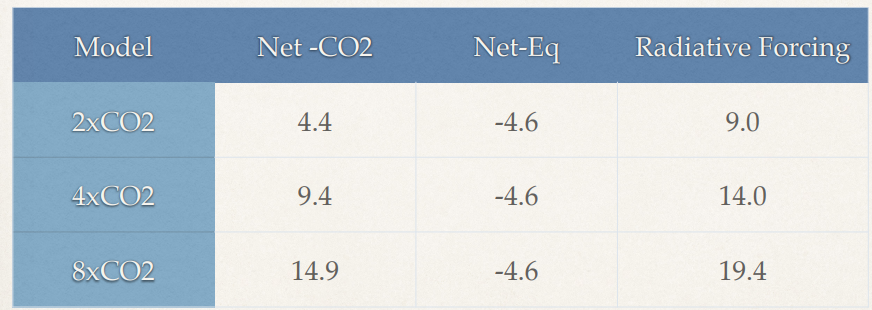
\includegraphics[width=0.3\textwidth]{uploads/image11.png}
	\end{center}
	\caption{Compute of radiative forcing.}
	\label{}
\end{wrapfigure}
Let's go back to the two layer model and compute the change in OLR:
\begin{equation}
	R\approx-\Delta OLR_S-\Delta OLR_1-\Delta OLR_2=
	-\Delta \tau[-2(1-\tau)\sigma T_S^4+(1-2\tau)\sigma T_1^4+\sigma T_2^4]
\end{equation}
Radiative forcing is the change in total radiative flux after a change in the absorbing properties of the atmosphere. Note that the radiative forcing depend on the vertical prole of temperature: for an isothermal prole $T_S=T_1=T_2$, hence:
$$R\approx0$$

Let’s try a case of radiative forcing due to an increase in greenhouse absorbers, using the tuned observed temperatures to the absorptivity parameter $\tau$ that we calculate to be 0.58 for the observed atmosphere. For the tuned value of $\tau=0.58$, we got that $T_S=288$ K, $T_1=275$ K, $T_2=230$ K let's compute the radiative forcing for an increase of 2\% of $\tau$, $\Delta \tau\approx 0.012$, then:
\begin{align*}
	\Delta OLR_S\approx 3.78 \\
	\Delta OLR_1\approx 0.65 \\
	\Delta OLR_2\approx-1.86
\end{align*}
So the total is $2.58$ W/m$^2$, so a small increase in absorption will decrease the outgoing $OLR$. Eventually the temperature at the ground will have to increase to adjust to the new situation. In short, radiative forcing is a direct measure of the amount that the Earth’s energy budget is out of balance. For the Earth’s climate system, it turns out that the level where this imbalance can most meaningfully be measured is the boundary between the troposphere and the stratosphere.

\begin{figure}[htpb]
	\centering
	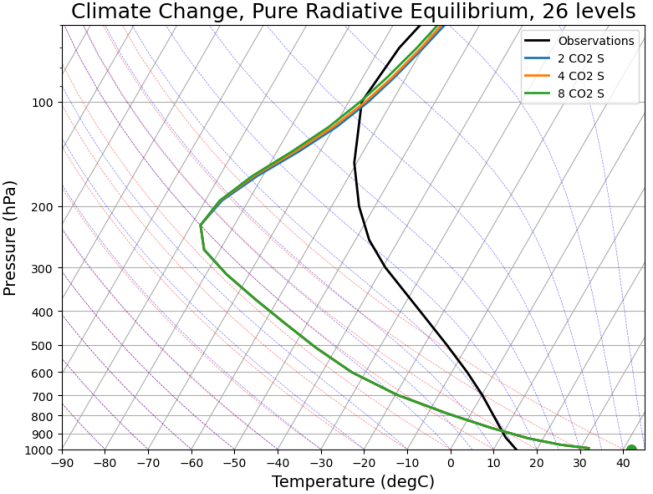
\includegraphics[width=0.4\linewidth]{uploads/Screenshot 2024-11-24 201309.png}
	\caption{Use a radiative-convective model, but keep the troposphere at the unperturbed equilibrium values.}

\end{figure}


\begin{figure}[htpb]
	\centering
	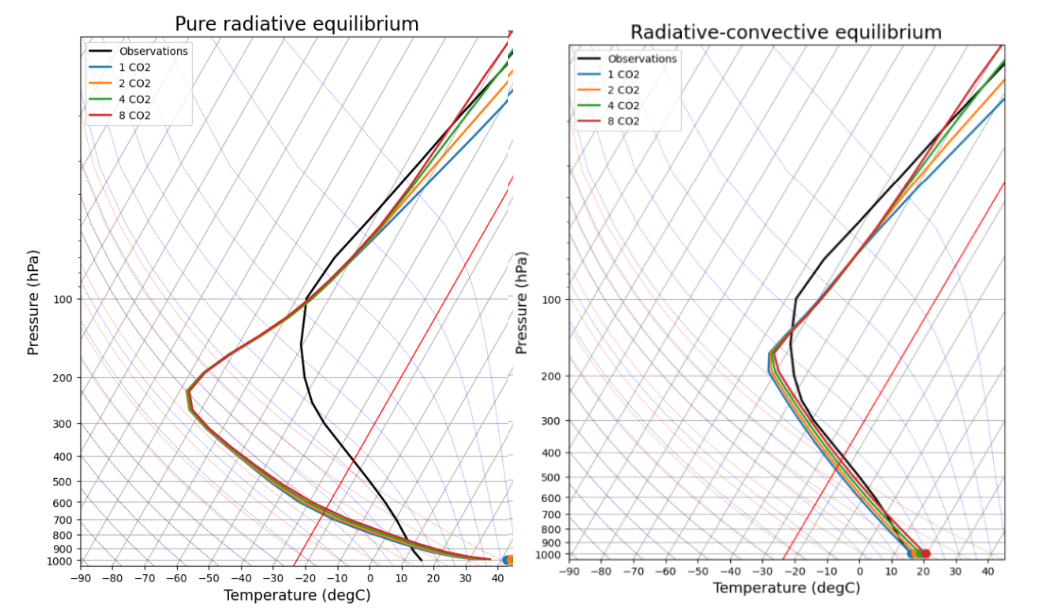
\includegraphics[width=0.5\linewidth]{uploads/Screenshot 2024-11-24 202614.png}
	\caption{Climate change}

\end{figure}
\subsection{Greenhouse feedback}
It refers to processes in the climate system that amplify or dampen the warming caused by the greenhouse effect.  The greenhouse effect is a natural process that warms the Earth’s surface by trapping heat from the Sun. Solar radiation reaches the Earth, and the surface absorbs and emits heat as infrared radiation. Greenhouse gases in the atmosphere, such as carbon dioxide (CO$_2$), methane (CH$_4$), water vapor (H$_2$O), and others, absorb and re-radiate this infrared radiation, warming the Earth's surface and lower atmosphere. Without this effect, the Earth's average temperature would be much colder, making it uninhabitable.

While the natural greenhouse effect is essential for life, human activities have enhanced it, primarily through the burning of fossil fuels, deforestation, and industrial processes, which increase the concentration of greenhouse gases. This intensification of the greenhouse effect has led to global warming and climate change, causing rising temperatures, melting ice, sea level rise, and more frequent extreme weather events.

Positive feedback mechanisms increase climate sensitivity, potentially leading to faster and more severe warming; negative feedback mitigates sensitivity, stabilizing the climate system.
The response parameter is:
\begin{equation}
	\lambda_0=\frac{\Delta R}{\Delta T_S}\quad \text{Wm$^{-2}$K$^{-1}$}
\end{equation}
The change is essentially constant, but we have not taken into consideration the possible effect of water, that is an important component in creating the opacity. Water vapor creates powerful feedback in the climate system.
\begin{figure}[htpb]
	\centering
	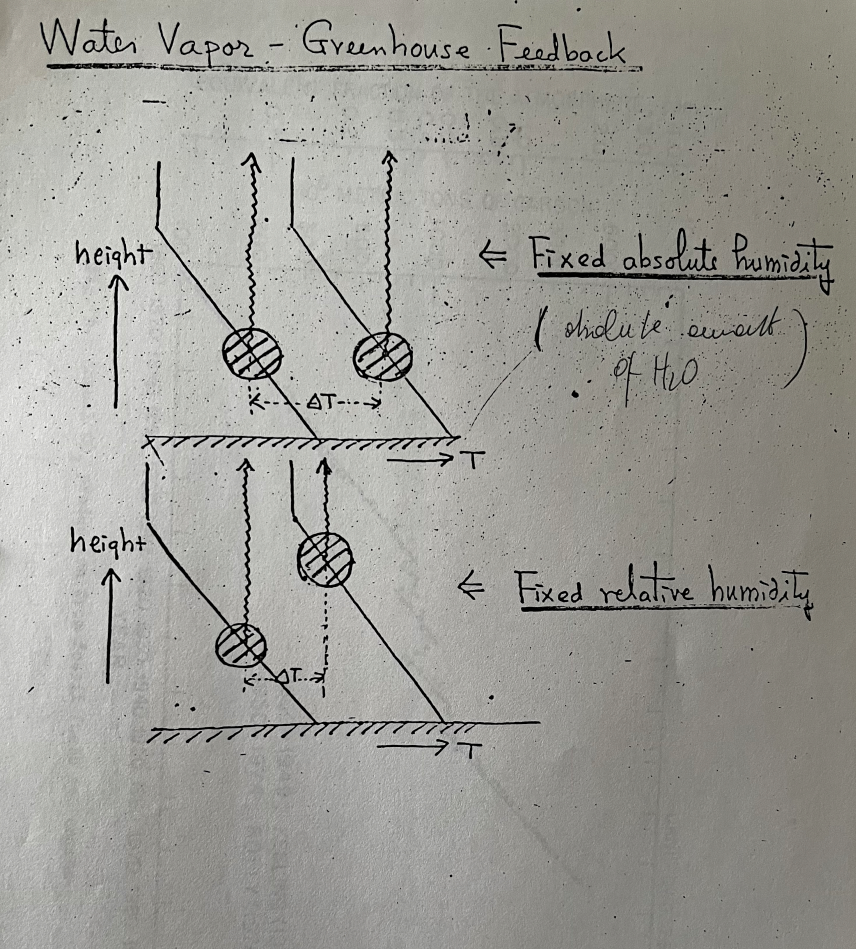
\includegraphics[width=0.25\linewidth]{uploads/Screenshot 2024-11-24 203149.png}
	\caption{Greenhouse feedback from Manabe 1981}

\end{figure}
\subsection{Water vapor feedback} Water vapor feedback is one of the most significant and well-understood feedback mechanisms in the Earth's climate system. It is a positive feedback that amplifies the warming caused by increased greenhouse gas concentrations.
An initial radiative forcing (for instance an increase in $CO_2$) generates a response in the surface temperature
\begin{equation}
	\Delta T_0=\frac{\Delta R}{\lambda_0}
\end{equation}
When the climate system starts to adjust it will see a new radiative forcing:
$$\Delta R+f\lambda_0\Delta T_0$$
where $f$ represents the  fraction of the initial radiative forcing that is transferred to the next cycle, after $n$ cycles we get
$$(1+f+f^2+f^3+\dots)\lambda_0\Delta T_0=\lambda_0\Delta T_0\sum_nf^n$$
if $f<1$ the sum can be done and we get: $$\Delta T=\Delta T_0\frac{1}{1-f}=g\Delta T_0$$
so the overall effect is positive if $f>0$ and the system gain $g$ is $g>1$.
This initial warming causes the surface temperature of the Earth to rise, leading to increased evaporation of water from oceans, lakes, and other sources. As more water enters the atmosphere in the form of vapor, the concentration of this potent greenhouse gas increases. Water vapor traps heat very effectively, which further warms the surface, creating a self-reinforcing cycle.
\begin{figure}[htpb]
	\centering
	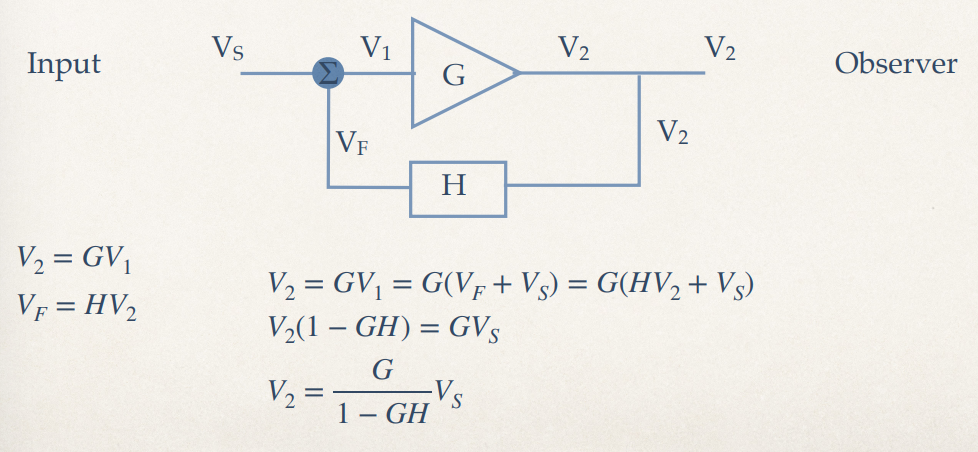
\includegraphics[width=0.38\linewidth]{uploads/13676.png}
	\caption{Feedback Loop, where $G$ amd $H$ are machines that determine $V_2$ that way.}

\end{figure}
The strength of water vapor feedback varies by region. It is most pronounced in the tropics, where the warm temperatures lead to significant evaporation and large increases in atmospheric water vapor. In contrast, in colder polar regions, the feedback is weaker because lower temperatures limit evaporation. This geographic variability means that water vapor feedback not only amplifies global warming but also contributes to differences in how warming manifests across the planet.\\
[0.25 cm]


In nature, as in a complex GCM, water vapor tends to increase as the air temperature warms. The main reason for this is that the saturation-specific humidity (i.e. how much water vapor the air can hold) increases strongly with temperature. We can parameterize this effect in the column model by insisting that the relative humidity remain fixed as the column warms. In the radiative-convective model, the relative water vapor adjusts rapidly.
\begin{figure}[htpb]
	\centering
	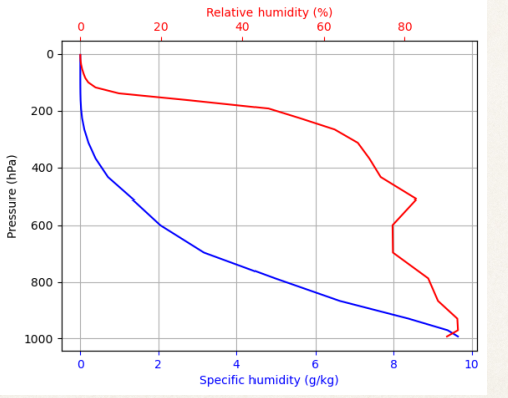
\includegraphics[width=0.28\linewidth]{uploads/image112.png}
	\caption{Relative water vapor in radiative-convective model.}

\end{figure}



The increasing temperature raises the saturation pressure allowing more water vapor to be present in the atmosphere. The previous perturbed experiment did not take into account this effect: it was basically a no-feedback simulation. To take into account the water-vapor feedback we have to constrain the model to keep its relative humidity fixed.\\
NB. Relative humidity is overall constant, specific humidity drops quickly with height and water vapor feedback increases the temperature of $\sim 2$°C.
\begin{figure}[htpb]
	\centering
	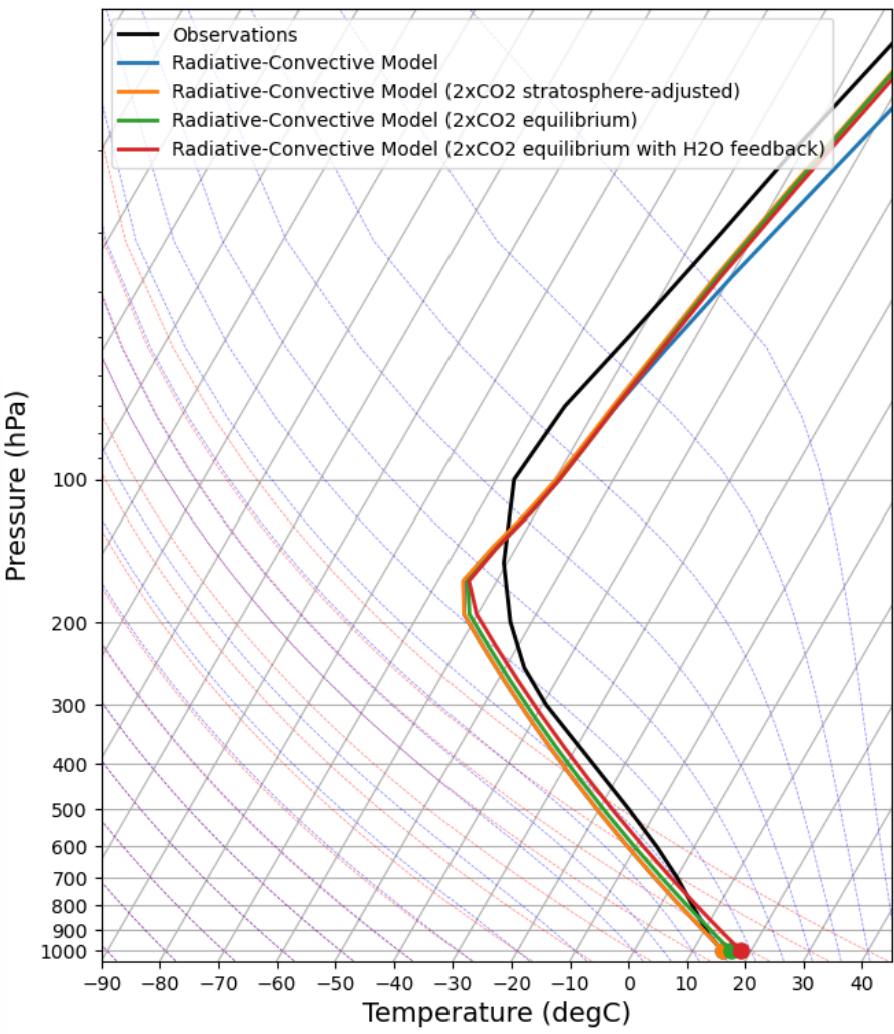
\includegraphics[width=0.4\linewidth]{uploads/23.png}
	\caption{Model with water-vapor feedback: relative humidity fixed.}

\end{figure}



Equilibrium Climate Sensitivity: the temperature at the
ground increases due to an increase of $CO_2$. $T$ of the new experiment is $2.98$ K, compare to the no-feedback experiment value of $1.31$ K. The gain
$$g=\frac{ECS}{ECS_{nofeedback}}>2$$
Water vapor feedback doubles the warming of the ground, this was the major result by Manabe and
Wetherald.\\
[0.4 cm]

In his 1964 paper, Manabe\cite{Manabe1964} focused on the interaction between radiation and convection in the atmosphere. The primary goal of the study was to understand how the atmosphere reaches a thermal equilibrium, considering both radiative and convective processes. Manabe developed a one-dimensional model that combined the radiative properties of the atmosphere with the effects of convective heat transfer. The model introduced the concept of \textit{convective adjustment}, a process where the atmosphere quickly adjusts to restore equilibrium when it is disturbed. Convective processes work to redistribute heat vertically, ensuring that the atmosphere can maintain thermal stability despite variations in surface temperatures and solar radiation. \\

Manabe demonstrated that the Earth's atmospheric temperature profile is governed by the balance between radiative cooling at higher altitudes and convective heating from the Earth's surface. The interaction between these two processes determines the temperature structure of the atmosphere, with convective adjustment helping to smooth out temperature gradients and reach a stable profile. Manabe also examined how changes in the concentration of greenhouse gases affect the temperature profile of the atmosphere. He showed that increased CO$_2$ leads to a warming of the lower atmosphere, as it enhances the greenhouse effect and reduces radiative cooling. One of the major conclusions of the study was that the atmosphere tends to reach a thermal equilibrium where the rates of incoming solar radiation and outgoing infrared radiation balance each other.




In his 1967 paper "Thermal Equilibrium of the Atmosphere with a Given Distribution of Relative Humidity"\cite{Manabe1967}, Manabe extended his previous work on the thermal equilibrium of the atmosphere by incorporating the effects of relative humidity into his climate model. Assuming a specific distribution of relative humidity (the amount of moisture in the air relative to its capacity at a given temperature) allowed him to examine how water vapor, as a greenhouse gas, influences the thermal structure of the atmosphere and contributes to the energy balance. One of the most important results was the identification of the water vapor feedback mechanism. Manabe showed that as the temperature of the atmosphere increases, the amount of water vapor also increases, since warmer air can hold more moisture. This additional water vapor enhances the greenhouse effect, leading to further warming, which in turn increases the water vapor content. This feedback loop amplifies the initial warming caused by other factors such as increased CO$_2$. The model demonstrated that the distribution of relative humidity significantly affects the vertical temperature profile of the atmosphere. Higher humidity in the lower atmosphere causes more water vapor to be present near the surface, which contributes to stronger greenhouse warming near the Earth's surface and a cooler stratosphere. The study showed how humidity influences both the radiative cooling and convective processes, ultimately shaping the thermal equilibrium of the atmosphere.\\

Building on his previous work, Manabe incorporated the concept of convective adjustment to account for the redistribution of heat and moisture in the atmosphere. The model showed that the presence of moisture, combined with the vertical heat transport due to convection, would lead to a different equilibrium state than in a dry atmosphere. This adjustment process, in turn, affects the thermal structure and stability of the atmosphere. Manabe also suggested that changes in the distribution of relative humidity, especially in response to global warming, could lead to nonlinear changes in the Earth’s climate. For example, increased moisture in the atmosphere as a result of warming could accelerate the warming process, as water vapor is a powerful greenhouse gas.
Initially general equations model for rain was produced when in a convective adjustment process, the specific humidity would be higher than the saturation of water vapor pressure, so the excess of humidity was considered rain. This was the first attempt to calculate in a physically consistent way the amount of rain. Rain is one of the major driving force for the atmosphere ( for the entire circulation).